%\title{My two column CV}
%
% tccv (two columns curriculum vitae) is a LaTeX class inspired by
% the template found at latextemplates.com by Alessandro Plasmati.
%
% Create by Nicola Fontana, the original files can be downloaded from:
% http://dev.entidi.com/p/tccv/
%
\documentclass{tccv}
\usepackage[english]{babel}
\usepackage{graphicx}
\usepackage{placeins}
\usepackage{amsmath}
\usepackage{amsfonts}

\begin{document}

\part{Michael. C. J. Kao}

%%%%%%%%%%%%%%%%%%%%%%%%%%%%%%%%%%%%%%%%%%%%%%%%%%%%%%%%%%%%%%%%%%%%%%%%
%% Personal contact and summary
%%%%%%%%%%%%%%%%%%%%%%%%%%%%%%%%%%%%%%%%%%%%%%%%%%%%%%%%%%%%%%%%%%%%%%%%


\vspace{0.5cm}
\personal
    [mkao006]
    {mkao006@gmail.com}
    {mkao006}

\section{Personal Summary}

Highly skilled data scientist with hands-on knowledge of the latest
statistic and machine learning techniques with a passion for
problem-solving and value creation.\\

Experience in productionising machine learning model on AWS and a
solid understanding of engineering practice.\\

I love diving, in water and data!


%%%%%%%%%%%%%%%%%%%%%%%%%%%%%%%%%%%%%%%%%%%%%%%%%%%%%%%%%%%%%%%%%%%%%%%%
%% Work experience and skills
%%%%%%%%%%%%%%%%%%%%%%%%%%%%%%%%%%%%%%%%%%%%%%%%%%%%%%%%%%%%%%%%%%%%%%%%

\section{Work experience}

\begin{eventlist}

\item{July 2018 -- Dec 2020}
  {\href{https://envato.com/}{Envato}, Melbourne, Australia}
  {Data Scientist}

  Pioneer of data science, promoting the adoption of advanced
  analytics and application of ML.

\item{July 2017 -- July 2018}
  {\href{http://www.fao.org/home/en/}{FAO of the United Nations}, Remote}
  {Consultant}

  Research on the application of Deep Learning models for detecting
  commodity market anomalies and future food crisis.
  
\item{November 2016 -- July 2017}
  {\href{http://deepblu.com/}{Deepblu Inc}, Taipei, Taiwan}
  {Senior Data Scientist}

  The technical lead of newly created data team reporting to senior
  management on everything about data.

\item{October 2011 -- October 2016}
  {\href{http://www.fao.org/home/en/}{FAO of the United Nations}, Rome, Italy}
  {Lead Statistician}

  R ambassador and project technical lead for the global Food Balance Sheet.\\
  
\item{June 2010 -- November 2011}
  {Ogilvy \& Mather, Auckland, New Zealand}
  {Data Analyst}


\end{eventlist}

%% \begin{figure}[h!] % use [hb] only if necceccary!
%%   \centering
%%   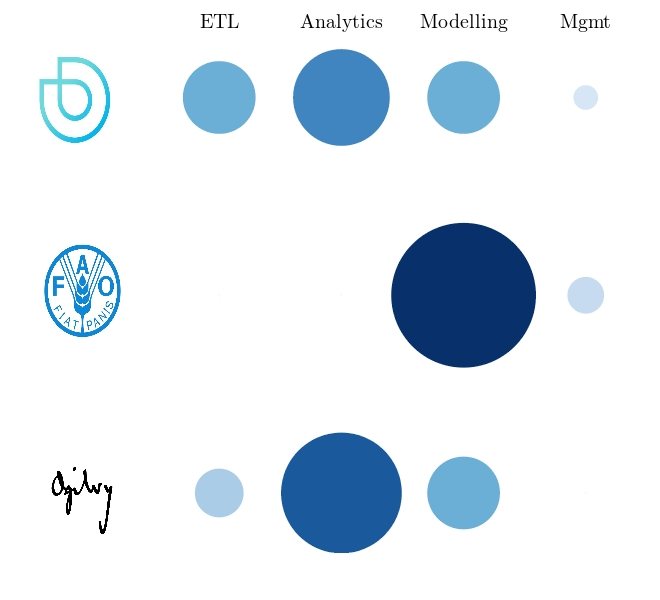
\includegraphics[width=9cm,height=7.5cm]{experience_association.jpeg}
%% \end{figure}

%%%%%%%%%%%%%%%%%%%%%%%%%%%%%%%%%%%%%%%%%%%%%%%%%%%%%%%%%%%%%%%%%%%%%%%%
%% software skills
%%%%%%%%%%%%%%%%%%%%%%%%%%%%%%%%%%%%%%%%%%%%%%%%%%%%%%%%%%%%%%%%%%%%%%%%

\section{Technical Skills}
\begin{factlist}
\item{Languages}
  {R, Python, Scala}
\item{Database}
  {SQL, PostGIS, Mongo, Redshift, BigQuery}
\item{Other}
  {Linux, Docker}
\item{AWS}
  {Lambda, S3, ECS, Sagemaker}
\end{factlist}



%%%%%%%%%%%%%%%%%%%%%%%%%%%%%%%%%%%%%%%%%%%%%%%%%%%%%%%%%%%%%%%%%%%%%%%%
%% Work Approach
%%%%%%%%%%%%%%%%%%%%%%%%%%%%%%%%%%%%%%%%%%%%%%%%%%%%%%%%%%%%%%%%%%%%%%%%

\section{Work Approach}

%% \begin{shadequote}[c]{Leonardo Da Vinci}
``Simplicity Is The Ultimate Sophistication``
%% \end{shadequote}

\vspace{0.1cm}

\begin{equation*}
  \min_{\beta \in \mathbb{R}^{d}}\left\{\|y - \mathbb{X}\beta \|_{2} + \lambda \|\beta \|_{1}\right\}\\
\end{equation*}

%% \begin{equation*}
%% {L(D)} = \min_{H \in {\cal H}} \ (\ L(H) + L(D|H) \ )
%% \end{equation*}

\vspace{0.1cm}

%% Where $R$ denotes the desired results and $P$ the problems at hand,
%% the coefficient $\beta$ represents the amount of effort dedicated to
%% each task.\\

%% In essense, never loose track of the ultimate goal, but allocate the
%% resources efficiently to achieve the best outcome.

%%%%%%%%%%%%%%%%%%%%%%%%%%%%%%%%%%%%%%%%%%%%%%%%%%%%%%%%%%%%%%%%%%%%%%%%
%% Award and scholarships
%%%%%%%%%%%%%%%%%%%%%%%%%%%%%%%%%%%%%%%%%%%%%%%%%%%%%%%%%%%%%%%%%%%%%%%%

%% \section{Awards \& Scholarships}

%% \begin{yearlist}
%% \item{2011}
%%      {RSVP and Nexus Award \newline for marketing insight}
%%      {}
%% \item{2011}
%%      {Master of Science Faculty Award with Scholarship}
%%      {}

%% \item{2010, 2011}
%%      {Senior Prize in Statistics}
%%      {}
%% \end{yearlist}


%%%%%%%%%%%%%%%%%%%%%%%%%%%%%%%%%%%%%%%%%%%%%%%%%%%%%%%%%%%%%%%%%%%%%%%%
%% Selected projects
%%%%%%%%%%%%%%%%%%%%%%%%%%%%%%%%%%%%%%%%%%%%%%%%%%%%%%%%%%%%%%%%%%%%%%%%

\section{Selected Projects}

\begin{yearlist}
\item{2018} {Diamond Analysis} {Scrapped diamond data from James Allen
  to build a pricing model to estimate how much I am about
  to get ripped off for an engagement ring.}

%% \item{2016} {DataKind Datadive Hackathon} {Prototyped a web app in
%%   Shiny to provide information on the animal density and observation
%%   trend.}
  
\end{yearlist}


\begin{figure}[h!] % use [hb] only if necceccary!
  \centering
  
\includegraphics[width=1cm,height=1cm]{../company_icon/envato.png}
\end{figure}

\begin{yearlist}

\item{2020} {Tag embedding} {Train embedding model on tag data for
  recommendation and automatd collection.}

\item{2020} {Churn analysis} {Analyse usage data to identify the path
  and point of churn.}
  
\item{2019} {Customer Segmentation} {Segment customers into multiple
  industries, providing a basis for personalised strategy.}

\item{2018} {Customer Lifetime Value} {Predict customer lifetime
  value using survival analysis to \textbf{ensure PPC campaigns
    provide an acceptable level of ROI}}

\end{yearlist}


\begin{figure}[h!] % use [hb] only if necceccary!
  \centering
  
\includegraphics[width=1cm,height=1cm]{../company_icon/deepblu.jpg}
\end{figure}

\begin{yearlist}
  %% \item{2017} {Data Pipeline Automation} {Employed Airflow to automate
  %%   and streamline the process of building the data lake.}

  \item{2017} {Hardware anormaly detection} {Applied isolation forest to detect
    anomalies in dive logs resulting from hardware faulty in dive
    computer to \textbf{improve the reliability of our product and the
      safety of diving}.}

  \item{2017} {Social Network Analysis}{Analysed the structure and
    connectivity of the market and devised an \textbf{acquisition
      strategy for exponential growth}.}
    
\end{yearlist}


\begin{figure}[h!] % use [hb] only if necceccary!
  \centering
  
\includegraphics[width=1cm,height=1cm]{../company_icon/fao.png}
\end{figure}

\begin{yearlist}
\item{2016} {The Reading Machine
  (\href{https://github.com/EST-Team-Adam/TheReadingMachine}{Github})}
  {Sentiment extraction and topic modelling of news article coupled
    with Recurrent Neural Network to forecast the commodity price. The
    purpose of the project is to \textbf{identify potential food
      crisis}.}

  
\item{2014} {Food Balance Sheet
  (\href{https://github.com/SWS-Methodology}{Github})} {An update to
  the latest methodology for the Food Balance Sheet (FBS). The work
  estimates \textbf{the global supply and demand of food} and as input
  to the \textbf{estimation of the number of undernourishment around
    the globe.}}
  
%% \item{2014} {Ensemble Imputation
%%   (\href{https://github.com/mkao006/sws\_imputation}{Github})} {Lead
%%   research on flexible and robust imputation methodology. An ensemble
%%   learning model was formulated to impute the global production of all
%%   agricultural products. \textbf{Over 200,000 time series were tested
%%     and imputed}.}

%% \item{2014} {Information Quality
%%   (\href{https://github.com/mkao006/sws\_flag}{Github})} {Use of
%%   entropy to measure relative information content of various data
%%   sources in order to \textbf{measure the quality of information} and
%%   construction of distribution for modelling.}

%% \item{2013}
%%      {Sentimental Mining
%%        (\href{https://github.com/mkao006/sofi\_twitter\_activity}{Github})}
%%      {Scrapped Twitter data for sentimental analysis in order to
%%        understand the reader response to flagship publication}

\item{2013}
     {R package: FAOSTAT
       (\href{http://cran.r-project.org/web/packages/FAOSTAT/index.html}{CRAN})}
     {An R package providing seamless integration to the FAO
       Statistics database.}
  
\end{yearlist}


\begin{figure}[h!] % use [hb] only if necceccary!
  \centering
  
\includegraphics[width=1cm,height=1cm]{../company_icon/ogilvy.jpg}
\end{figure}

\begin{yearlist}

%% \item{2011} {What Teacher Shortage?
%%   (\href{http://nzdmawards.co.nz/winners-archive/2011-winners-gallery/ministry-of-education-what-teacher-shortage}{RSVP
%%     Award})} {Forecasted demand and supply of teachers and analysed
%%   the labour force to provide insights on the reality of the teaching
%%   force. The RSVP and Nexus prize was awarded for \textbf{confirming
%%     that the teacher shortage was truly over and assisted in new
%%     policy formulation}.}

  
\item{2011} {Marketing Optimisation Analysis} {The project estimated the effects of
  various advertising channel in order to assess the respective
  efficiency and effectiveness. The estimations were then employed to
  optimise the allocation of the marketing budget for a large retail
  banking client. The result was a \textbf{79\% improvement in
    customer acquisition over the existing budget}.}

\end{yearlist}

\begin{yearlist}
\item{2011}
     {Finding High Achievers}
     {The project identified segments of individuals who are high
       achievers from students of economically deprived
       background. The uses of the PRIM algorithm \textbf{pinpoint a
         segment with a 70\% completion rate as opposed to the pool
         average of 41\%}. This resulted in improved utilisation of
       public funding.}
  
\end{yearlist}

\vspace{10cm}

%%%%%%%%%%%%%%%%%%%%%%%%%%%%%%%%%%%%%%%%%%%%%%%%%%%%%%%%%%%%%%%%%%%%%%%%
%% Personal interests
%%%%%%%%%%%%%%%%%%%%%%%%%%%%%%%%%%%%%%%%%%%%%%%%%%%%%%%%%%%%%%%%%%%%%%%%

\section{Interests}

\begin{factlist}
\item{Hobbies} {Scuba diving, basketball, boxing, yoga, cooking and
  travelling}
\end{factlist}

\FloatBarrier
  \centering
  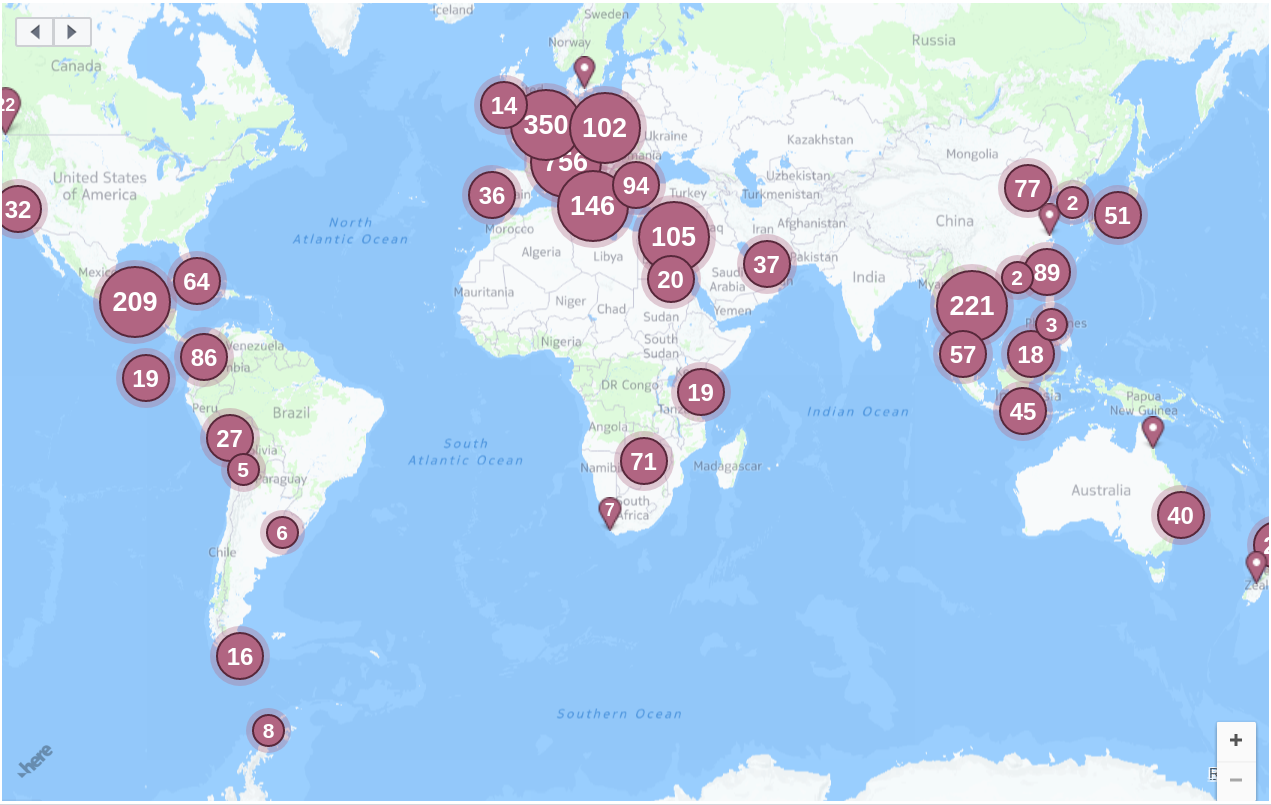
\includegraphics[scale = 0.2]{places_I_have_been_2.png}
  \textit{Places I have visited}
\FloatBarrier

%%%%%%%%%%%%%%%%%%%%%%%%%%%%%%%%%%%%%%%%%%%%%%%%%%%%%%%%%%%%%%%%%%%%%%%%
%% Education
%%%%%%%%%%%%%%%%%%%%%%%%%%%%%%%%%%%%%%%%%%%%%%%%%%%%%%%%%%%%%%%%%%%%%%%%

%% \vspace{5in}
\section{Education}

\begin{yearlist}
  
\item[University of Auckland]{2010 -- 2012}
     {M.Sc. in Statistic}
     %% {SNM-GARCH: A semi-parametric mixture extension to GARCH modelling}
{}

\item[University of Auckland]{2009 -- 2010}
     {B.A. (1st Class Hons.) \newline in Statistics}
     %% {Complex Demodulation/Remodulation of Electricity Consumption Time Series.}
{}

\item[University of Auckland]{2005 -- 2009}
  {B.A. \& B.Sc}
  {}
  %% {Majored in Economics, \newline Finance and Statistics}

\end{yearlist}


\end{document}
